%kelompok 2
%Achmad Fatahillah(1154004)
%Ilga Anne Tri J.S(1154045)
%Maulyanda(1154008)
%Mefi Frinkazela Nikica(1154073)
%Simon Sorba Manangi(1154019)

\section{Variabel}
Pada sebagian besar dari bahasa pemrograman, nama suatu variabel
menjelaskan suatu nilai dengan tipe data tertentu 
dan menempati alamat memory yang pasti.
Variabel menyimpan data atau nilai yang dilakukan selama program dieksekusi,
Nilai suatu variabel tersebut dapat diganti-ganti, namun pada tipe data selalu tetap ada.
Tidak demikian dengan sebuah python dimana tipe datanya dapat diubah-ubah
secara dinamis\cite{suparno2013komputasi}.

Variabel merupakan entitas yang memiliki nilai dan nilai tersebut berbeda satu sama yang lain. Variabel mengalokasikan memori untuk menyimpan nilai - nilai nya.
Hal ini berarti ketika saat anda membuat variabel maka anda memesan beberapa atau sebuah ruang di memori tersebut. 
Variabel dapat digunakan untuk menyimpan bilangan bulat, desimal juga karakter.
Python sangat mementingkan indentasi, sehingga kita perlu melakukan indentasi secara konsisten. 
Indentitas tersebut dipermudah dengan menggunakan tombol Tab dan dimulai dari kolom pertama untuk setiap blok baru.

Variab membutuhkan pengenal atau bisa disebut dengan identifier yg didefinisikan oleh pemrograman. Tanda pengenal atau identifier memiliki aturan-aturan dalam penulisannya seperti:
\begin{enumerate}
\item
harus diawali huruf atau di garis bawah
\item
tidak menggunakan aritmatika
\item
jika terdiri dari dua kata atau lebih,makan antar katanya tidak boleh menggunakan spasi
\item
tidak boleh menggunakan kata-kata yang sudah ada arti khususnya dalam bahasa Python
\item
penggunaan huruf kecil dan besar harus dibedakan
\item
panjang maksimal yaitu 32 karakter
\end{enumerate}

Variabel merupakan nama yang menunjukkan nilai tertentu. Dalam Pyton, untuk membentuk variabel cukup memberi nama pada nlai yang kita inginkan. Statement yang melakukan hal tersebut disebut assignment.
\begin{verbatim}
>>> pesan = “Hi, Apa kabar D43A”
>>> n = 20
>>> pi = 3.14159
\end{verbatim}

Contoh diatas menunjukkan tiga buah assigment. Contoh pertama memberi nilai 
``Hi, Apa kabar D43A'' pada variabel pesan, 
kedua memberi nilai 20 pada variabel n, dan ketiga memberi sebuah nilai 3.14159 pada variabel pi.
\cite{utami2004logika}

Variabel akan memiliki tipe  sesuai dengan nilainya.
\begin{verbatim}
>>>type(mesg)
<Type ‘string’>
>>> type (n)
<type ‘int’>
>>> type (pi)
<type ‘float>
\end{verbatim}

Contoh lainnya:
\begin{verbatim}
>>>menit=59
>>>menit/60
0
\end{verbatim}
Nilai yang telah diberikan oleh si variabel menit itu adalah 59, jika kita hitung, maka pembagiannya 59 oleh 60 akan menghasilkan angka 0,9833333. Tapi, dalam Python memberi nilai 0. Hal ini terjadi karena bahasa pemrograman Python menggunakan pembagian integer. Jika kedua operan adalah integer, makan hasilnya itu harus berupa integer juga, dan pembagian integer itu selalu dibulatkan ke bawah

Nilai variabel dapat tampil dengan perintah print:
\begin{verbatim}
>>> print pesan
Hi, Apa kabar D43A
>>> print n
20
>>>print pi
3.14159
\end{verbatim}

Akan tetapi, jika pada command-line, maka dapat langsung dipanggil nama variabel tersebut :
\begin{verbatim}
>>> pesan
Hi, Apa kabar D43A
\end{verbatim}

Perintah dari print juga dapat memberi lebih dari satu nilai dalam satu baris:
\begin{verbatim}
>>> print “Nilai dari pi adalah “,pi
Nilai dari pi adalah 3.14159
\end{verbatim}

koma untuk memisahkan nilai dan variabel.\cite{utami2004logika}

Ada 2 cara untuk membuat variabel. Cara yang pertama yaitu variabel langsung dengan nilai disebut dengan inisialisasi. Sedangkan cara yang kedua dengan memasukkan nilai pada variabel yang biasa disebut penempatan.\cite{santoso2009bahasa}

Variabel python tidak perlu untuk melakukan deklarasi eksplisit untuk memesan ruang memori. Deklarasi tersebut terjadi secara otomatis ketika menetapkan nilai ke variabel nya.
Tanda sama (=) dapat digunakan untuk memberikan nilai pada variabel.

Operan di sebelah kiri operator =  nama dari variabel dan operan di sebelah kanan operator = nilai yang disimpan dalam variabel
Python memiliki lima tipe data standar -
Nomor
Tali
Daftar
tupel
Kamus

Variabel pada Python memiliki beberapa aturan seperti :
\begin{itemize}
\item
Case Sensitive : penggunaan huruf besar dan huruf kecil yang dibedakan.
\item
Harus dimulai dengan underscore (\_) atau huruf biasa, setelah itu dapat diikuti dengan huruf, angka atau underscore (\_).
\item
Tidak boleh mengandung karakter special seperti !,@,\#,\$ dan lainnya.
\item
Hanya dapat menggunakan suatu variable setelah kita memberikan nilai ke dalamnya atau telah dilakukan assignment.
\item
Setiap variable akan menyimpan referensi ke suatu objek dalam memory.\cite{santoso2009bahasa}
\end{itemize}

Variabel adalah sebuah nama yang selalu menunjukkan nilai tertentu. Dalam bahasa pemrograman Python, untuk membentuk sebuah variabel itu cukup hanya memberi nama pada nilai yang akan dibuat. Ini disebut dengan Assignment.
Contoh : 
\begin{verbatim}
>>>pesan="Halo, Semuanya"
\end{verbatim}
Contoh di atas membuktikan bahwa itu adalah sebuah assignment, yang memberi kan sebuah nilai \"Halo, Semuanya\".\cite{utami2004logika}

contoh lainnya:
\begin{verbatim}
>>> c = 2 # c bilangan bertipe integer
>>> print c
2
>>> c = c * 2.0 # Sekarang c bilangan bertipe float
>>> print c
4.0
\end{verbatim}

ke suatu object dalam memory. Untuk lebih jelasnya
dapat kita lihat contoh berikut ini :
\begin{verbatim}
>>> a = 2
>>> b = 3
>>> a,b = b,a
>>> a
3
>>> b
2
>>>
\end{verbatim}

Beberapa bentuk if adalah sebagai berikut :
\begin{verbatim}
a. if tunggal
if x == 1:
print ‘x bernilai 1’
b. if dengan else
if x == 1:
print ‘x bernilai 1’
else:
print ‘x tidak bernilai 1’
c. if dengan pilihan if lainnya
if x == 1:
print ‘x bernilai 1’
elif x == 2:
print ‘x bernilai 2’
else:
print ‘x tidak bernilai 1 atau 2’
d. if di dalam if
if x == 1:
if y == 1:
print ‘x dan y bernilai 1’
\end{verbatim}

Tulisan a = 2 artinya kita memberi nilai pada variabel a dengan angka 2 yang bertipe integer
(bilangan bulat). Statemen berikutnya adalah melakukan operasi perkalian a ∗ 2.0 lalu hasilnya
disimpan pada variabel yang sama yaitu variabel a. Dengan demikian nilai a yang lama
akan diganti dengan nilai a yang baru, yaitu yang berasal dari operasi yang terakhir.
Sebagai Konsekuensi atau hasil dari operasi yang dirancang atau dibuat tersebut, 
sekarang variabel a memiliki tipe data float, 
suatu tipe dapat berkaitan dengan bilangan pecahan atau desimal. 
Nilai variabel b menghasilkan nilai 4.0 atau empat\ref{pythonvariable}.
\begin{figure}[ht]
    \centerline{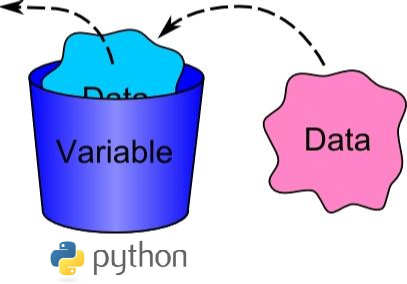
\includegraphics[width=0.25\textwidth]{figures/pythonvariable.png}}
    \caption{gambar yang menggambarkan keadaan variabel pada python}
    \label{pythonvariable}
    \end{figure}

Tanda dari pagar (\#) menyatakan awal dari suatu komentar. Komentar adalah bagian dari
script program python yang tidak akan dieksekusi oleh interpreter. 
Python mementingkan indentasi, sehingga perlu indentasi yang konsisten. Indentasi dipermudah sesuai penggunaan
tombol Tab dan dimulai dari kolom pertama untuk setiap blok baru. 
Bahasa pemrograman Python suatu fasilitas  shell di Linux, sehingga kita untuk mencoba penggunaan
Python secara leluasa. Lokasi instalan Python default pada distribusi Linux.
keunggulan Python adalah :
\begin{enumerate}
\item
Python is powerful and fast = suatu kumpulan modul-modul yang sangat baik dan dapat menangani secara praktis setiap domain masalah
\item
Python plays well with others = Python bisa berintegrasi dengan Component Object Model (COM) 
\item
Python runs everywhere = versi Python berjalan di .NET, Java Virtual Machine dapat melihat bahwa sumber yang sama dapat berjalan tanpa perubahan berarti pada setiap sistem operasi tersebut.
\item
Python is Open = Python dilisensi open source membuat Python digunakan dan disebarkan secara free,
\item
Python is friendly and easy to learn = Dokumentasi yang lengkap merupakan salah satu fasilitas Python yang disenangi penggunanya. Apabila pembaca melakukan instalasi Python
\end{enumerate}

Dalam menulis program, akan menggunakan code yang pernah kita  buat atau ditulis sebelumnya, pasti
kita gunakan kembali, dengan beberapa nilai berbeda.
 
Tentu saja tidak mungkin menuliskan kembali kode yang ingin dipanggil ulang tersebut.
Solusinya, supaya dapat dikelompokan kode-kode yang sering dipanggil ulang dalam suatu kelompok.

Selain itu dapat memecah masalah-masalah yang besar  menjadi masalah-masalah yang lebih kecil.
Dalam C atau bahasa pemrograman lain, biasanya digunakan istilah function.

Kemampuan dari python dalam mengelola tipe data sangat baik. Untuk melakukan pendeklarasian suatu variabel dapat dilakukan secara langsung tanpa menyebutkan tipe - tipe data, ini yang membedakan sebuah python dengan bahasa lain. Python akan menentukan tipe-tipe data tersebut secara otomatis. Python juga dapat mendukung konversi dan perhitungan antar semua tipe data tersebut dengan keakuratan yang tinggi. Python membagi sebuah tipe data ke dalam 2 jenis bilangan (semua tipe yang berhubungan dengan angka murni) dan string. Untuk tipe data dalam rumpun bilangan termasuk di dalamnya adalah integer, long, float, oktal, hexadimal dan bilangan kompleks. Hal-hal yang harus diperhatikan :
\begin{itemize}
\item
Untuk suatu bilangan oktal dan hexa masing-masing diawali dengan 0 dan 0x
\item
Untuk bilangan panjang diakhiri menggunakan karakter dari l ataupun J
\item
Untuk bilangan float dapat menggunakan e atau E pada eksponensial
\item
Untuk bilangan kompleks dapat dibagi menjadi bagian real dan imajiner, dan diakhiri dengan j atau J Operator untuk tipe dalam rumpun bilangan.\cite{utamipemrograman}
\end{itemize}

\subsection{Membuat Perubah Variabel}
Variabel atau perubah memiliki suatu symbol yang dapat dimuati oleh sembarang himpunan dari bilangan tersebut. Dalam pengertian dari komputasi sebuah nama dapat digunakan untuk menyimpan suatu nilai dengan kapasitas tertentu dan alamat tertentu dalam sebuah memori komputer tersebut. Variabel merupakan pendaftaran dari tipe data bagi variabel itu, konstanta dan parameter sering digunakan untuk sebuah program agar dapat mempunyai alamat penyimpanannya dan kapasitas dari data nya dalam memori komputer. Dalam membuat variabel kita hindari spasi dan dapat menggunakan sebuah karakter khusus, selain itu nama dalam sebuah kata cadangan Python (seperti input, eval, if, elif, for, def, dan lain-lain) tidak dapat menjadi variabel.\cite{irfani2016bahan}

Nama variabel atau disebut juga dengan identifier dalam bahasa pemrograman Python juga dapat berupa kumpulan dari huru (letter) maupun angka (digit) yang dengan cara membedakan huruf kecil dan juga huruf besar, Karakter pertama pada identifier harus berupa huruf dan juga perlu diketahui bahwa penggunaan karakter garis bawah itu juga dapat digunakan.
Kesalahan sintax akan muncul apabila dalam penamaan sebuah variabel itu tidak sesuai dengan aturan yang ada.
Contoh :
\begin{verbatim}
>>>876swafm="Radio Swa"
SyntaxError: invalid syntax
>>>more$=1000000
\end{verbatim}
SyntaxError: invalid syntax
Baris pertama itu salah, karena pada 876swafm karakter pertamanya itu bukanlah huruf. Pada baris ketiga juga salah karena pada more\$ berisi karakter dolar.

Tidak seperti pemrograman pada lainnya, variabel pada Python tidak harus dideklarasikan secara eksplisit. Pendeklarasian variabel terjadi secara otomatis ketika kita memberikan sebuah nilai pada suatu variabel. Tanda sama dengan (=) dapat digunakan untuk memberikan value/nilai pada suatu variabel. Operan di sebelah kiri dari tanda (=) adalah nama variabel, sedangkan operan yang sebelah kanan dari tanda (=) adalah nilai yang diberikan pada variabel.\cite{utamipemrograman}

\begin{verbatim}
>>>harga = 100
>>>diskon = 30
>>>harga - diskon
70
\end{verbatim}

Pada contoh di atas tersebut, 100 dan 30 adalah suatu nilai yang diberikan untuk variabel harga dan variabel diskon itu. Sedangkan pernyataan dari harga-diskon akan menghitung selisih antara harga dengan diskon. Variabel juga dapat menyimpan suatu nilai berupa teks (dibaca string).

\begin{verbatim}
>>>a = 'sekolah'
>>>b = 'dasar'
>>>a + b
'sekolahdasar'
\end{verbatim}

Variabel juga bisa menyimpan dua nilai string atau lebih dengan menggunakan operator (+).

\begin{verbatim}
>>>c = 'Py' + 'thon'
>>>c
'Python'
\end{verbatim}

Jika kita telah melakukan penilaian pada variabel, kita dapat menggunakan variabel tersebut pada yang lainnya.

\begin{verbatim}
>>>a = 2
>>>a = a + 3
>>>a
5
\end{verbatim}

Selain itu, juga dapat memberikan sebuah nilai untuk beberapa variabel.

\begin{verbatim}
>>>p=q=r=1
>>>p
1
>>>q
1
>>>r
1
\end{verbatim}

Selain itu, kita dapat memberikan beberapa nilai untuk beberapa variabel (disebut multiple assignment).

\begin{verbatim}
>>>x, y, z = 1, 2, 'belajar Python'
>>>x
1
>>>y
2
>>>z
'belajar Python'
\end{verbatim}

Bentuk lain dari sebuah contoh di atas, kita juga dapat menggunakan tanda kurung-buka atau kurung-tutup.

\begin{verbatim}
>>>(x, y, z) = (1, 2, 'Belajar Sebuah Python')
Cara di atas, dapat juga kita gunakan untuk pertukaran nilai variabel.
>>>(x, y) = (10, 20)
>>>x
10
>>>y
20
>>>(x, y) = (y, x)
>>>x
20
>>>y
10
\end{verbatim}

Contoh-contoh  pada prompt Python adalah sebagai berikut 

\begin{verbatim}
>>> a = 1
>>> a
1
>>> b = 2
>>> b
2
>>> c = a + b
>>> c
3
>>> d = a - b
>>> d
-1
>>> print ‘Nilai d adalah : ‘, d
Nilai d adalah : -1
>>> print ‘Nilai c adalah : ‘, c
Nilai c adalah : 3
>>> e
Traceback (most recent call last):
File “<stdin>”, line 1, in ?
\end{verbatim}

\begin{verbatim}
Python yang sederhana : 
$ vi contoh-script-01.py
#! /usr/bin/python
a = 1
print ‘Nilai a adalah : ‘ , a
simpan script Anda dengan : 
:wq
\end{verbatim}

Secara default, script Python disimpan dengan ekstensi .py

\subsection{Aturan Penulisan Variabel}
\begin{itemize}
\item
Nama variabel bisa diawali dengan menggunakan huruf atau garis bawah (\_), contoh: nama, \_nama, namaKu, nama\_variabel.
\item
Karakter selanjutnya dapat menggunakan berupa huruf, garis bawah (\_) atau angka, contoh: \_\_nama, n2, nilai1.
\item
Karakter pada nama variabel bersifat sensitif (case-sensitif). Artinya huruf besar dan kecil dibedakan. Misalnya, variabel\_Kita dan variabel\_kita, keduanya adalah variabel yang berbeda.
\item
Nama variabel tidak boleh menggunakan kata kunci yang sudah ada dalam python seperti if, while, for, dsb.
\end{itemize}

\subsection{Menghapus Variabel}
Ketika sebuah atau suatu variabel tidak dibutuhkan lagi, maka kita bisa menghapusnya dengan fungsi del().
Contoh:

\begin{verbatim}
>>> nama = "petanikode"
>>> print nama
petanikode
>>> del(nama)
>>> print nama
Traceback (most recent call last):
  File "<stdin>", line 1, in <module>
NameError: name 'nama' is not defined
>>>
\end{verbatim}

Pada perintah terakhir, kita akan mandapatkan NameError. Artinya variabel tidak terdapat di dalam memori alias sudah dihapus.

\subsubsection{Penempatan variable pada yang semestinya}
Misalkan sebuah data pribadi dapat berisi nama, alamat, umur, tempat lahir, tanggal lahir, indeks prestasi kumulatif akan memberikan 6 (enam) buah variabel tipe datanya.
\begin{figure}[ht]
    \centerline{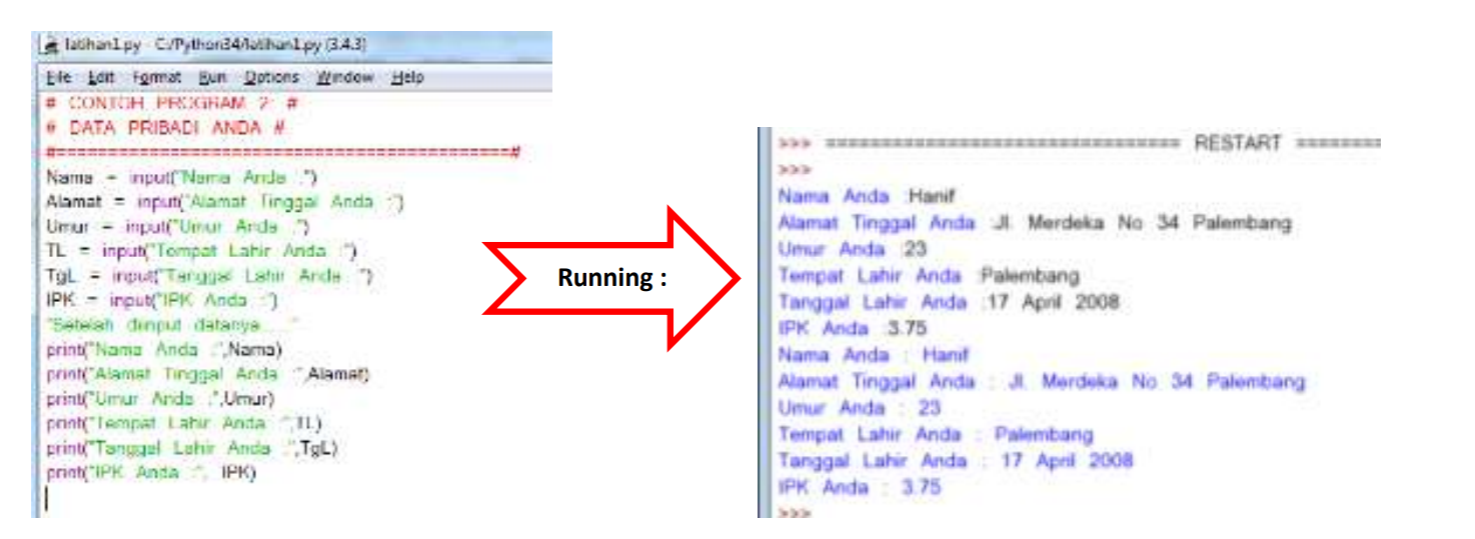
\includegraphics[width=1\textwidth]{figures/tipedatastring.png}}
    \caption{Tampilan Contoh Input/Output Tipe Data String}
    \label{tipedatastring}
    \end{figure}

\begin{figure}[ht]
    \centerline{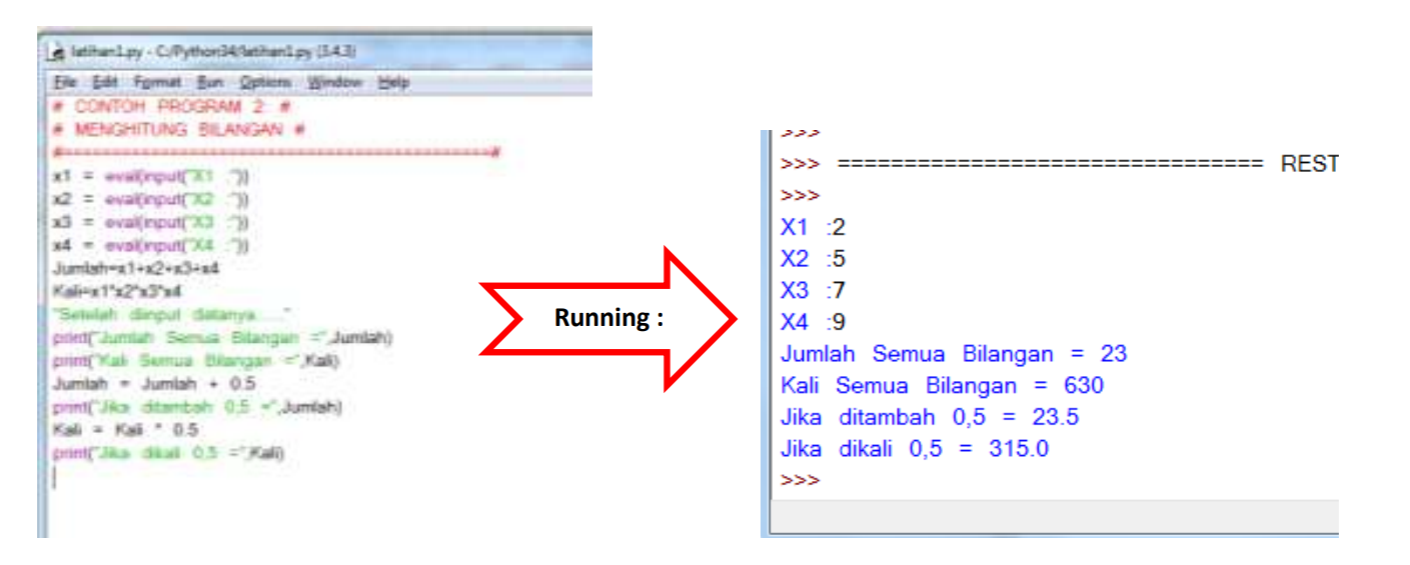
\includegraphics[width=1\textwidth]{figures/tipedatabilangan.png}}
    \caption{Tampilan Contoh Input/ Output Tipe Data Bilangan}
    \label{tipedatabilangan}
    \end{figure}

Pada Gambar 2.2 \ref{tipedatabilangan} terlihat input/output pada tipe data bilangan dengan hasil yang berbeda tipe bilangan yaitu tipe dari integer (bilangan bulat) atau float (bilangan berkoma).\cite{irfani2016bahan}

\subsubsection{Memberikan nilai ke dalam variable}
Lakukan konstanta dari permasalahan berikut! Menjumlahkan hasil dari total harga pada saat konsumen membeli beberapa barang.

Langkah 1: Inisiasi Persoalan 
Variabel konstanta input :  
kode\_barang, nama\_barang, harga\_satuan\_barang, 
jumlah\_barang\_beli, total\_harga\_transaksi = 0 
Proses :  harga\_beli\_barang = harga\_satuan\_barang * jumlah\_barang\_beli 
total\_harga\_transaksi = harga\_beli\_barang + total\_harga\_transaksi
Output :  total\_harga\_transaksi

Langkah 2: Menetapkan Tipe Data 
kd\_brg, nama\_brg bertipe data string 
jum\_brg merupakan tipe data integer harga\_satuan, harga\_beli, total\_hrg\_brg bertipe data float 

Langkah 3 : Kode program
\begin{figure}[ht]
    \centerline{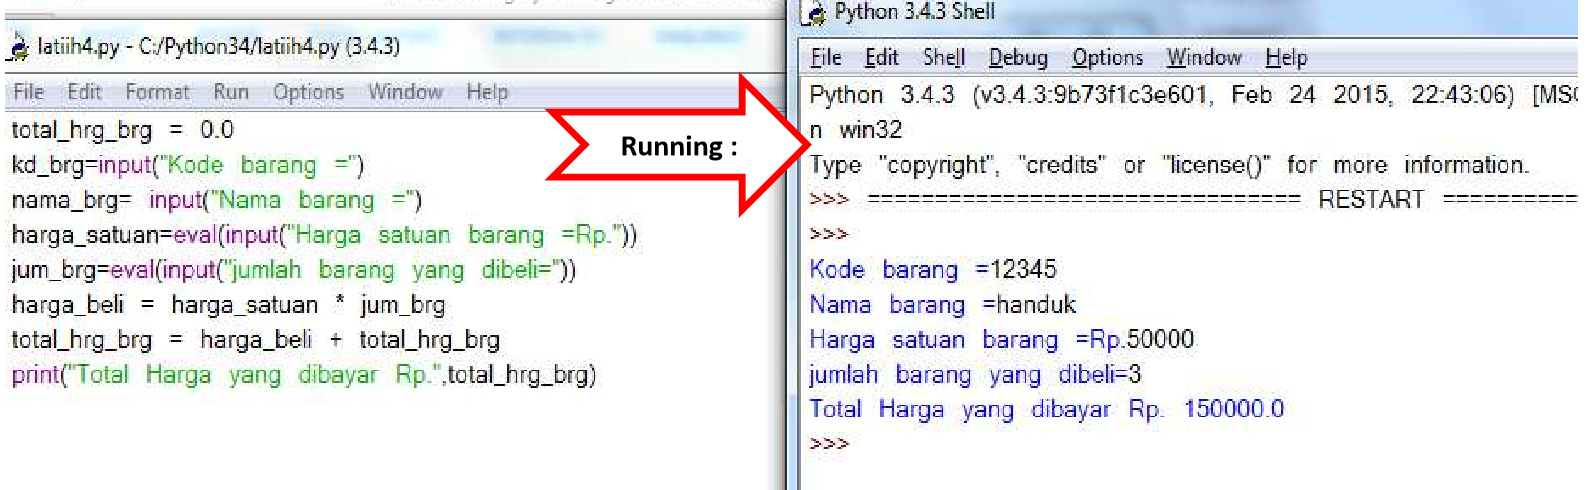
\includegraphics[width=0.50\textwidth]{figures/code.png}}
    \caption{kode program}
    \label{code}
    \end{figure}
  
\subsubsection{Mencetak nilai dalam variable} 
Mencetak nilai dari sebuah variabel menggunakan pernyataan print, perhatikan 
contoh berikut ini. 
\begin{figure}[ht]
    \centerline{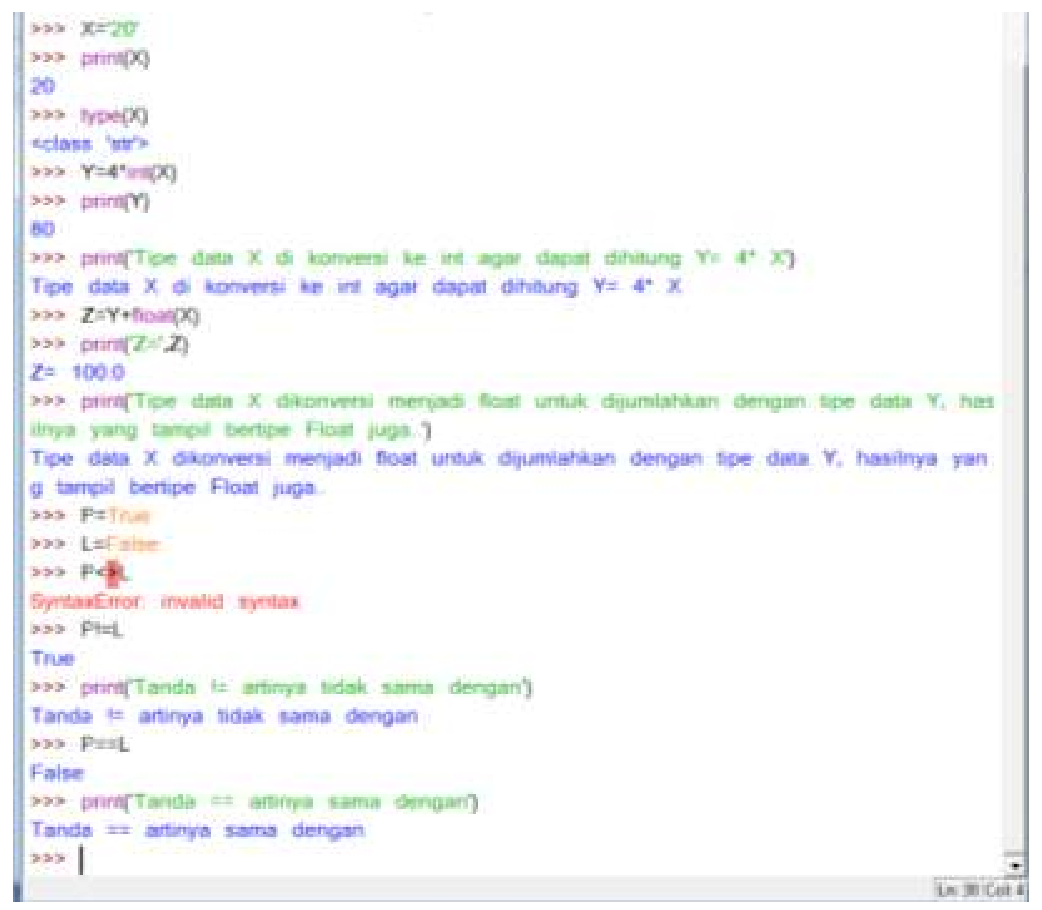
\includegraphics[width=0.25\textwidth]{figures/konversi.png}}
    \caption{Tampilan Contoh Konversi Tipe Data String dan Integer}
    \label{Tipe Data String dan Integer}
    \end{figure}

\subsection{Bilangan integer dan float}
Perbedaan tipe bilangan ini bisa dapat jadi potensi menimbulkan masalah. 
Ini contohnya
\begin{verbatim}
>>> 1/2 # bilangan integer dibagi bilangan integer
0 # tentu saja kita ini keliru, mestinya 0.5
>>> 1/2.0 # bilangan integer dibagi bilangan float
0.5 # kali ini hasilnya tepat
\end{verbatim}

\subsection{List}
List adalah sejumlah atau suatu object yang dipisahkan oleh tanda koma (,) dan diapit oleh kurung siku
([ ]). Begini contohnya:
\begin{verbatim}
>>> a = [1.0, 2.0, 3.0] # membuat list
>>> a.append(4.0) # tambahkan 4.0 kedalam list
>>> print a
[1.0, 2.0, 3.0, 4.0]
>>> a.insert(0,0.0) # sisipkan 0.0 pada posisi 0
>>> print a
[0.0, 1.0, 2.0, 3.0, 4.0]
>>> print len(a) # menentukan panjang list
5
\end{verbatim}
Jika kita memberikan suatu statemen c = b, maka itu tidak berarti bahwa variabel c terpisah dengan
variabel a. Di python, statemen tersebut dapat diartikan hanya sebagai pemberian nama lain
(alias) kepada variabel a. Artinya, perubahan yang terjadi baik itu di a ataupun di b, maka hasil
akhir mereka berdua akan sama saja. Setiap perubahan terjadi di c akan berdampak di b.
Untuk meng-copy a secara independen, gunakan statemen d = a[:]. 
Berikut adalah beberapa contoh lambang atau tanda untuk melengkapi setiap statement pada
variabel yang ada\ref{operate}.
\begin{figure}[ht]
    \centerline{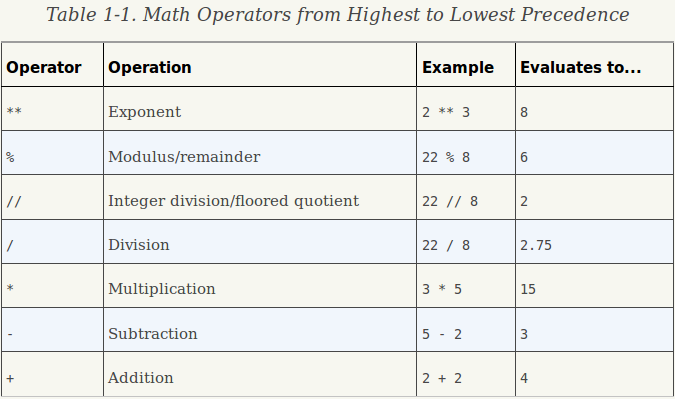
\includegraphics[width=0.25\textwidth]{figures/operate.png}}
    \caption{gambar tanda operasi pada python}
    \label{operate}
    \end{figure}
